\newpage
\chapter{Interactive application for factor graphs: EFG$\_$GUI}
\label{chap:GUI}

EFG$\_$GUI is a graphical user interface designed to manipulate medium-size factor graphs. It is essentially composed by two parts: EFG$\_$GUI.exe and EFG$\_$GUI.html.
EFG$\_$GUI.exe implements an Http server, listening for the user requests and satisfying them using the EFG library.
When you double click  EFG$\_$GUI.exe, EFG$\_$GUI.html is automatically launched, using your default browser. EFG$\_$GUI.html is an html interface through which the user communicates its need to the executable file.
\\
When you close from the browser an EFG$\_$GUI.html window, the executable is automatically terminated: never close the application directly.
\\
Always keep EFG$\_$GUI.exe, EFG$\_$GUI.html , src/, img$\_$GUI/, image/ in the same folder.
\\
\\
When you run EFG$\_$GUI.exe, it will appear a window similar to Fig. \ref{fig:home}.
The white region on the bottom it is a dashboard that will contain the structure you will work on, while the one on the top a list of always available commands that you can click. In the following of this Chapter, every command  of the interface will be commented.
\\
EFG$\_$GUI exploits the html5 technology, but it does not require a connection: the front-end .html is executed locally by your browser.

\begin{figure}
	\centering
	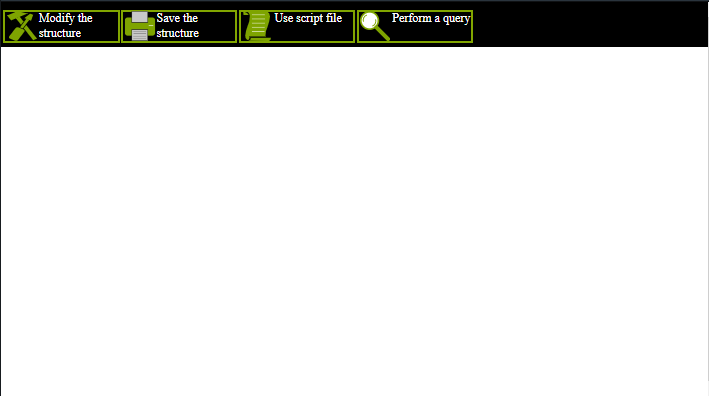
\includegraphics[width= 0.49 \columnwidth]{../src/Chapter_additional/04_EFG_GUI/image/img_00.png}
	\caption{The home page of the interface.}
	\label{fig:home}
\end{figure} 

\section{Modifying commands}

This set of commands alter the structure of graph you are working on. By clicking the top left button, left part of Figure \ref{fig:modif_toolbar}, the set of modifying commands will appear, right part of Figure \ref{fig:modif_toolbar}.

\begin{figure}
	\centering
\begin{tabular}{ll}
\begin{minipage}[t]{0.49\textwidth}
	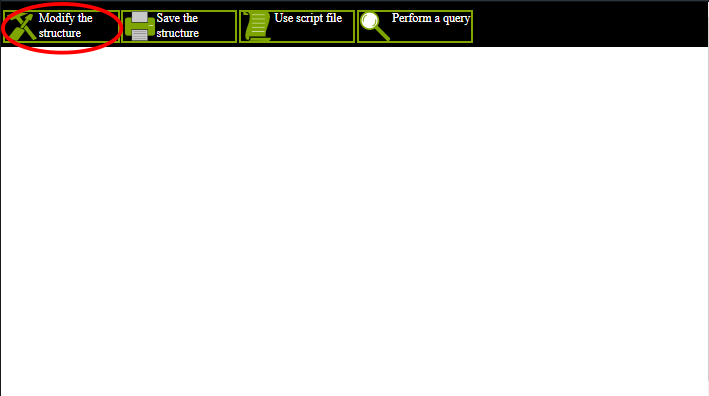
\includegraphics[width= \columnwidth]{../src/Chapter_additional/04_EFG_GUI/image/img_01.png}
\end{minipage}
 &
\begin{minipage}[t]{0.49\textwidth}
	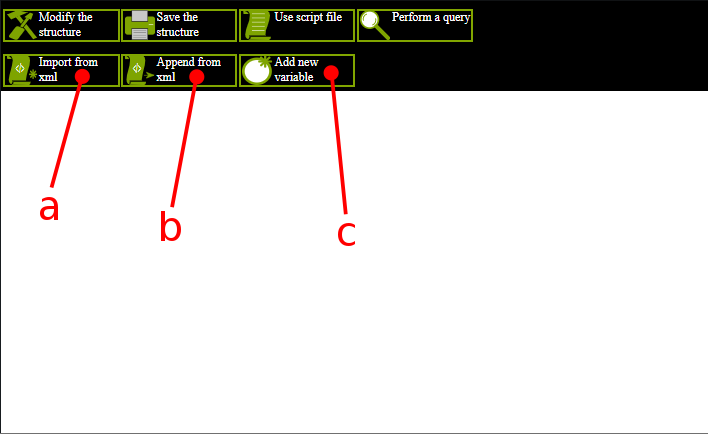
\includegraphics[width= \columnwidth]{../src/Chapter_additional/04_EFG_GUI/image/img_02.png}
\end{minipage}
\end{tabular}
	\caption{The location of the button enabling the modifying commands is indicated on the left. On the right the tool bar with the modifying commands.}
	\label{fig:modif_toolbar}
\end{figure}

\subsubsection{Import command}

By clicking command a of the toolbar in the right part of Figure \ref{fig:modif_toolbar}, you can import a new structure from an xml file (such files must be compliant with the format described in Chapter \ref{00_XML_format}): a pop-up will appear that lets you browser the folders on your pc for finding the xml you are interested in. The current structure is deleted and the new one is imported.

\subsubsection{Append command}

By clicking command b of the toolbar in the right part of Figure \ref{fig:modif_toolbar}, you can append the structure described by an xml file (such files must be compliant with the format described in Chapter \ref{00_XML_format}) to the current one: a pop-up will appear that lets you browser the folders on your pc for finding the xml you are interested in. In the back end, $Node\_factory::\_\_Absorb$ is invoked. In case the actual structure is empty, the effect of this command is the same of the Import command.

\subsubsection{Create variable command}

By clicking command c of the toolbar in the right part of Figure \ref{fig:modif_toolbar}, you can add a new variable: a first pop-up will appear asking you for the name to give to the new variable and a second one will ask you the $Dom$ size. The name of the new variable must be different from any other variable present at the time of calling the Create variable command (when you give an already used name, the variable is simply not created). When the variable is successfully created, it is not attached to the actual graph: it starts to exists in the dashboard as a separate node. Then, you can create some potentials that connects the new variable to some others already in the graph, see the buttons described in \ref{sec:GUI:isolated}.

\section{Global query commands}

This set of commands perform some queries on the entire graph present in the dashboard. By clicking the top right button, left part of Figure \ref{fig:global_query}, this set of commands will appear, right part of Figure \ref{fig:global_query}.

\begin{figure}
	\centering
\begin{tabular}{ll}
\begin{minipage}[t]{0.49\textwidth}
	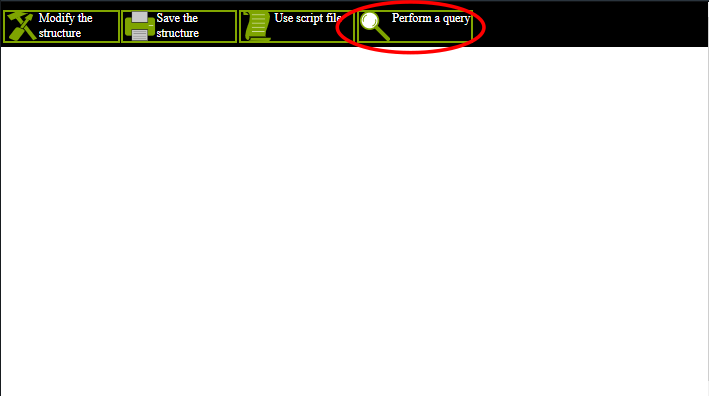
\includegraphics[width= \columnwidth]{../src/Chapter_additional/04_EFG_GUI/image/img_03.png}
\end{minipage}
 &
\begin{minipage}[t]{0.49\textwidth}
	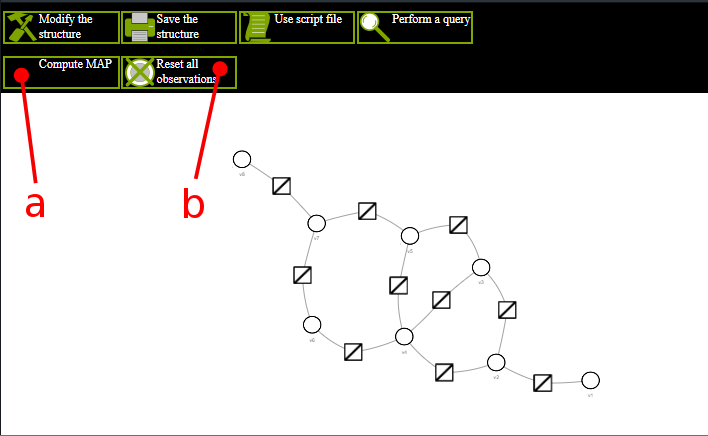
\includegraphics[width= \columnwidth]{../src/Chapter_additional/04_EFG_GUI/image/img_04.png}
\end{minipage}
\end{tabular}
	\caption{The location of the button enabling the global query commands is indicated on the left. On the right the tool bar with the global query commands.}
	\label{fig:global_query}
\end{figure}

\subsubsection{Compute MAP command}
\label{sec:GUI:MAP_com}

By clicking command a of the toolbar in the right part of Figure \ref{fig:global_query}, you can ask for a MAP estimation (Section \ref{sec:00:MAP}) of the set of variables that currently are hidden in the current graph. After back-end ends the MAP computation, the visualization of the graph in the dashboard is updated, adding to the labels of the hidden variables the value resulting from the MAP estimation.

\subsubsection{Reset observations command}

By clicking command b of the toolbar in the right part of Figure \ref{fig:global_query}, you can delete all the evidences of the graph, i.e. set the of evidences $\mathcal{O}$ (Section \ref{sec:00:PREL}) to an empty set. Consequently all the variables in the model will be treated as hidden. Clearly, any probabilistic query results previously computed (MAP estimation, Section \ref{sec:GUI:MAP_com}, or marginal computations, button d described in Section \ref{sec:GUI:hidden}) is deleted.

\section{Save command}

Clicking the command indicated in Figure \ref{fig:save} you can save the actual graph into an xml file (the format described in Chapter \ref{00_XML_format} is assumed). A pop-up will appear asking you the name of the file were you want to save the graph in the dashboard. You can give as prefix to the name of the file both relative and absolute paths.

\begin{figure}
	\centering
	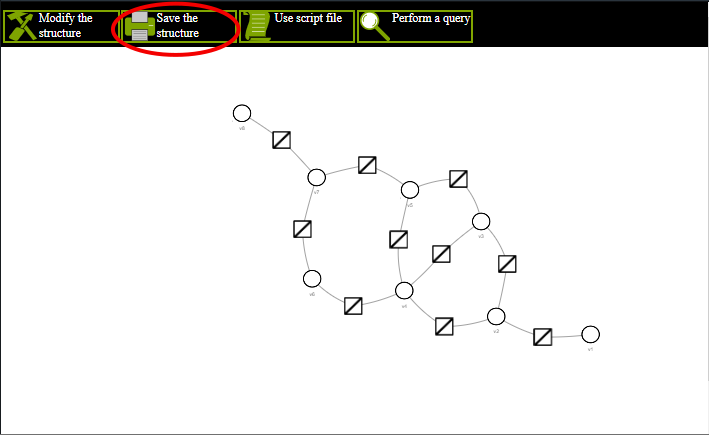
\includegraphics[width= 0.49 \columnwidth]{../src/Chapter_additional/04_EFG_GUI/image/img_05.png}
	\caption{The saving command.}
	\label{fig:save}
\end{figure} 

\section{Script command}

Clicking the command indicated in Figure \ref{fig:script} you can execute the list of commands indicated in a script file. A pop-up will appear letting you select the scripting file. Such a script file must be a simple plain text file. Each row of that file is interpreted as a command to perform.
Any accepted instruction must begin with a letter and can have a certain number of options. the options must be separated by the special character $\$$.
For instance '$P\$v\$name_1\$v\$name_2\$c\$T$' is a command having $P$ as initial symbol and two options of type $v$ and an additional one of type $c$.
The list of accepted commands is reported in table \ref{tab:GUI:commands}.

\begin{figure}
	\centering
	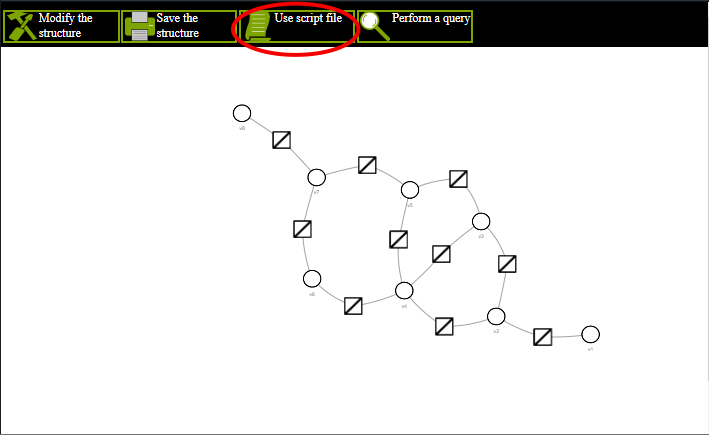
\includegraphics[width= 0.49 \columnwidth]{../src/Chapter_additional/04_EFG_GUI/image/img_06.png}
	\caption{the script execution command.}
	\label{fig:script}
\end{figure} 

\begin{table}[]
\begin{tabular}{|l|l|}
Syntax & Description \\
\hline
$X$ & 
\begin{minipage}[t]{0.8\textwidth}
Delete all the variables in the dashboard.
\end{minipage} \\
\hline
$X\$f\$S$ & 
\begin{minipage}[t]{0.8\textwidth}
Import the graph described by the file at the $f$ location.
\end{minipage}  \\
\hline
$X\$p\$S\$f\$S$ & 
\begin{minipage}[t]{0.8\textwidth}
Import the graph described by the file at the $p/f$ location: $p$ is simply the folder were to read the file.
\end{minipage} \\
\hline
$A\$f\$S$ &
\begin{minipage}[t]{0.8\textwidth}
 Append to the current structure, the graph described by the file at the $f$ location.
\end{minipage} \\
\hline
$A\$p\$S\$f\$S$ &
\begin{minipage}[t]{0.8\textwidth}
 Append to the current structure, the graph described by the file at the $p/f$ location: $p$ is simply the folder were to read the file.
\end{minipage} \\
\hline
$R\$f\$S$ &
\begin{minipage}[t]{0.8\textwidth}
 Print the current graph into an xml file at the $f$ location.
\end{minipage} \\
\hline
$V\$v\$S\$s\$S\$v\$S\$s\$S$ &
\begin{minipage}[t]{0.8\textwidth}
 Create new isolated variables: one for every specified pair $v-s$. In each pair $v$ represents the name to give to the new variable, while $s$ is its $Dom$ size.
\end{minipage} \\
\hline
$V\$v\$S\$s\$S\$v\$S\$s\$S$ &
\begin{minipage}[t]{0.8\textwidth}
 Create new isolated variables: one for every specified pair $v-s$. In each pair $v$ represents the name to give to the new variable, while $s$ is its $Dom$ size. There is no limit to the number of variables you can create with a single command.
\end{minipage} \\
\hline
$O\$v\$S\$n\$N\$v\$S\$n\$N$ &
\begin{minipage}[t]{0.8\textwidth}
 Add the specified variable to the set of evidences. Each pair $v-n$ represents the additional evidence to add: $v$ specifies the name of the variable that is observed and $n$ the value assumed. There is no limit to the number of variables you can specify.
\end{minipage} \\
\hline
$O$ &
\begin{minipage}[t]{0.8\textwidth}
 Delete all the evidences, i.e. $\mathcal{O} = \emptyset$.
\end{minipage} \\
\hline
$I\$v\$S\$v\$S$ &
\begin{minipage}[t]{0.8\textwidth}
 Computes the marginals of the specified set of variables: the $v$ options are the name of the variables whose marginals must be computed. There is no limit to the number of variables you can specify.
\end{minipage} \\
\hline
$M$ &
\begin{minipage}[t]{0.8\textwidth}
 Computes the MAP estimation of the entire hidden set $\mathcal{H}$.
\end{minipage} \\
\hline
$B\$f\$S$ &
\begin{minipage}[t]{0.8\textwidth}
 Executes the series of command specified in the script file at the location specified by $f$. Indeed, you can call a script file from another.
\end{minipage} \\
\hline
$P\$v\$S\$s\$S$ &
\begin{minipage}[t]{0.8\textwidth}
 Add a unary simple shape potential involving variable $v$ and whose image is described by a file (with the format describe by equation (\ref{eq:00:XML_struct:shape_txt})) at $s$.
\end{minipage} \\
\hline
$P\$v\$S\$s\$S\$w\$N$ &
\begin{minipage}[t]{0.8\textwidth}
 Add a unary exponential potential involving variable $v$ and whose image is described by a file (with the format describe by equation (\ref{eq:00:XML_struct:shape_txt})) at $s$, with a weight equal to $w$.
\end{minipage} \\
\hline
$P\$v\$S\$v\$S\$s\$S$ &
\begin{minipage}[t]{0.8\textwidth}
 Add a binary simple shape potential involving the variables specified by options $v$ and whose image is described by a file (with the format describe by equation (\ref{eq:00:XML_struct:shape_txt})) at $s$.
\end{minipage} \\
\hline
$P\$v\$S\$v\$S\$s\$S\$w\$N$ &
\begin{minipage}[t]{0.8\textwidth}
 Add a binary exponential shape potential involving the variables specified by options $v$ and whose image is described by a file (with the format describe by equation (\ref{eq:00:XML_struct:shape_txt})) at $s$, with a weight equal to $w$.
\end{minipage} \\
\hline
$P\$v\$S\$v\$S\$c\$S$ &
\begin{minipage}[t]{0.8\textwidth}
 Add a binary simple shape potential involving the variables specified by options $v$ that can be: a simple correlating shape in case $c=T$ or an anti-correlating one in case $c=F$. 
\end{minipage} \\
\hline
$P\$v\$S\$v\$S\$c\$S\$w\$N$ &
\begin{minipage}[t]{0.8\textwidth}
 Add a binary exponential shape potential involving the variables specified by options $v$ that can be: an exponential correlating shape in case $c=T$ or an anti-correlating one in case $c=F$,  with a weight equal to $w$.
\end{minipage} \\
\hline
\end{tabular}
\caption{List of accepted commands. $S$ indicates a string value, while $N$ a numerical one.}
\label{tab:GUI:commands}
\end{table}

\section{Variable specific commands}

This series of commands appear in the menu on the left of the dashboard, left part of Figure \ref{fig:inspector}, when you click on a variable in the dashboard. They handle variable specific commands. According to the kind of clicked variable, different options will be available. Anyway, for any variable clicked, the inspector represented will show at least the name of the clicked variable as well as its $Dom$ size, see again left part of Figure \ref{fig:inspector}. Then, additional commands may appear according to the kind of clicked variable, see the right picture of Figure \ref{fig:inspector}. 

\begin{figure}
	\centering
\begin{tabular}{ll}
\begin{minipage}[t]{0.49\textwidth}
	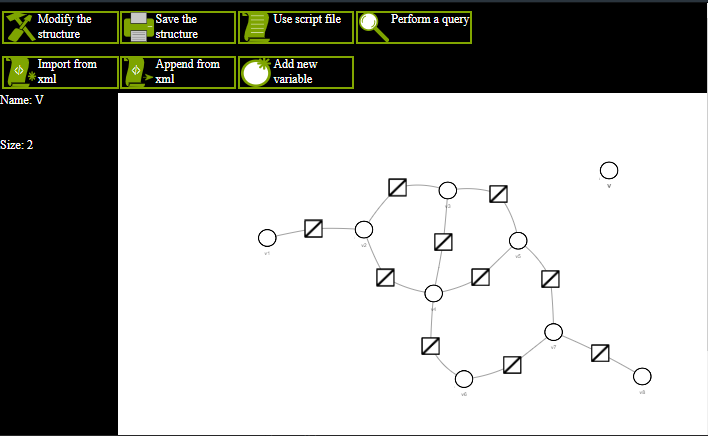
\includegraphics[width= \columnwidth]{../src/Chapter_additional/04_EFG_GUI/image/img_07.png}
\end{minipage}
 &
\begin{minipage}[t]{0.49\textwidth}
	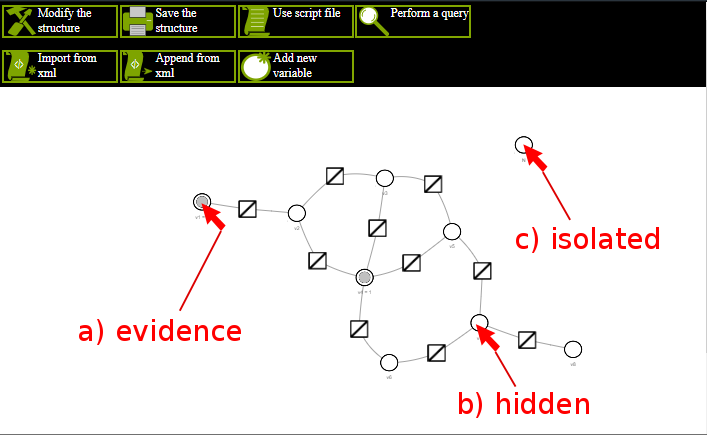
\includegraphics[width= \columnwidth]{../src/Chapter_additional/04_EFG_GUI/image/img_08.png}
\end{minipage}
\end{tabular}
	\caption{The inspector on the left part of the left picture appears when you click on a variable in the dashboard. The right part of the picture reports the three kind of variables that can be clicked: a) a variable in the evidence set, b) an hidden variable that is part of the graph and c) an isolated variable.}
	\label{fig:inspector}
\end{figure}

\subsection{Isolated variable}
\label{sec:GUI:isolated}

When you click on an isolated variable (case c in the right picture of Figure \ref{fig:inspector}) the command indicated in the left part of Figure \ref{fig:isolated} appears, but only in case you previously clicked an hidden variable in the graph (case b in the right picture of Figure \ref{fig:inspector}). Indeed, in such a case the indicated button allows you to add a factor going from the previously clicked variable and the isolated one. After click that button, the options indicated in the right part of Figure \ref{fig:isolated} will show up. More precisely, button a and b will appear only in the case the two clicked variables have the same $Dom$ size, while the c button will always appear. Button a allows you to add a simple correlating potential (the one created by using Potential$\_$Shape::Potential$\_$Shape(const std::list<Categoric$\_$var*>$\&$ var$\_$involved, const bool$\&$ correlated$\_$or$\_$not = true)), while button b an anti correlating one (the one created by using Potential$\_$Shape::Potential$\_$Shape(const std::list<Categoric$\_$var*>$\&$ var$\_$involved, const bool$\&$ correlated$\_$or$\_$not = false)). After clicking one of that two button, a pop-up will ask you to insert the value of the weight: if you submit a value equal to 0 a simple shape (refer to Figure \ref{fig:00:factor_kind}) correlating/anti-correlating factor will be created, while if you pass a positive number an exponential (refer to Figure \ref{fig:00:factor_kind}) correlating/anti-correlating factor, with the passed value for the weight, will be inserted to the graph. If you click on button c, firstly a pop-up asking for the value of the weight will appear and after that you will be asked to navigate the folders searching for a file that describes the values in the image of the potential to insert (the same format indicated in equation (\ref{eq:00:XML_struct:shape_txt}) is assumed). Also in this case, when passing a null weight, a simple shape factor is inserted, while an exponential factor is created in the opposite case.


\begin{figure}
	\centering
\begin{tabular}{ll}
\begin{minipage}[t]{0.49\textwidth}
	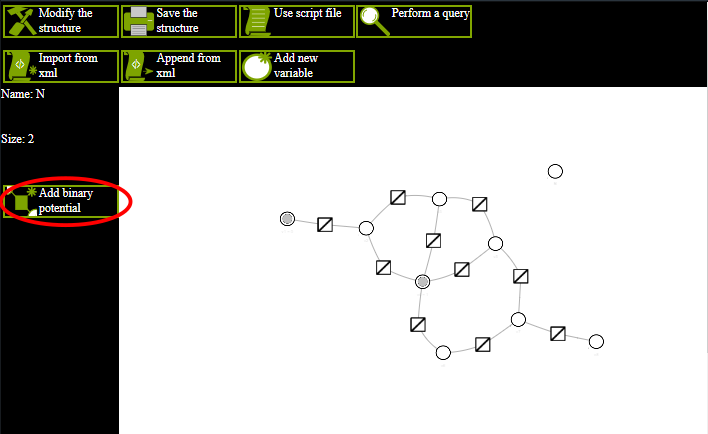
\includegraphics[width= \columnwidth]{../src/Chapter_additional/04_EFG_GUI/image/img_09.png}
\end{minipage}
 &
\begin{minipage}[t]{0.49\textwidth}
	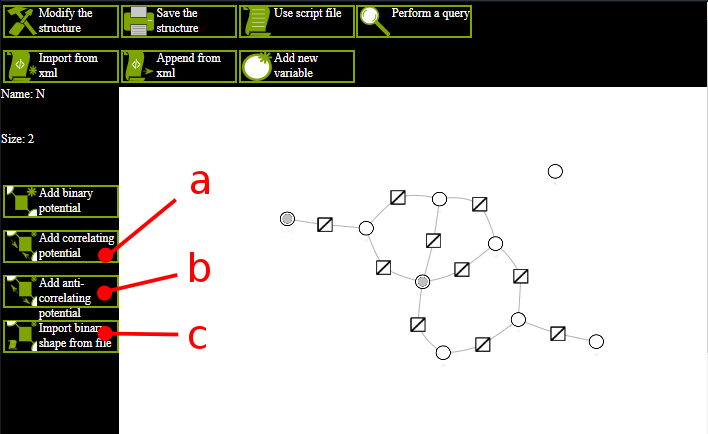
\includegraphics[width= \columnwidth]{../src/Chapter_additional/04_EFG_GUI/image/img_10.png}
\end{minipage}
\end{tabular}
	\caption{The inspector options for an isolated variable.}
	\label{fig:isolated}
\end{figure}

\subsection{Hidden variable in the model}
\label{sec:GUI:hidden}

When you click on an hidden variable (case b in the right picture of Figure \ref{fig:inspector}) the commands indicated in the left part of Figure \ref{fig:hidden} may appear. Buttons a, b and d will always appear, while button c will appear only in the case that you have previously clicked another hidden variable. Button c allows you to add a binary factor involving the clicked variable and works exactly as the one indicated in Section \ref{sec:GUI:isolated}.
\\
Button a allows you to make the clicked a variable a new observation: a pop-up will ask you to insert the observed value to assume. In case such a value is inconsistent with the $Dom$ size of the clicked variable, the instruction is ignored. 
\\
Button b allows you to add a unary potential involving the clicked variable. A pop-up will ask you to insert the value of the weight and then you will be asked to indicate the file that contains the values in the image of the potential (refer to equation (\ref{eq:00:XML_struct:shape_txt})).
\\
Button d allows you to ask for the marginal probability of the clicked variable (conditioned to all the evidences). After clicking that button, the back-end process will compute the marginals and will communicate them to the interface. After that, if you click again that variable, an histogram showing the marginals will appear. By clicking one of the bar in that histogram a pop-up will show you the exact value of probability that bar represents, see the right part of Figure \ref{fig:hidden}. Results about the marginals are saved for future inspection of that variable. Clearly, when the structure is modified or the evidences are changed, the information about the marginal probabilities are deleted.


\begin{figure}
	\centering
\begin{tabular}{ll}
\begin{minipage}[t]{0.49\textwidth}
	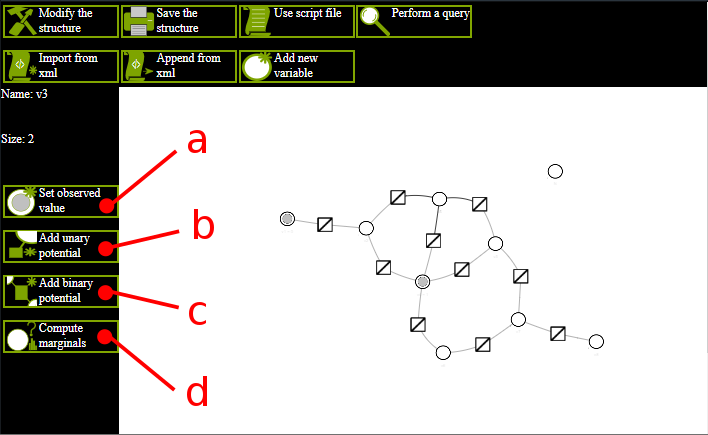
\includegraphics[width= \columnwidth]{../src/Chapter_additional/04_EFG_GUI/image/img_11.png}
\end{minipage}
 &
\begin{minipage}[t]{0.49\textwidth}
	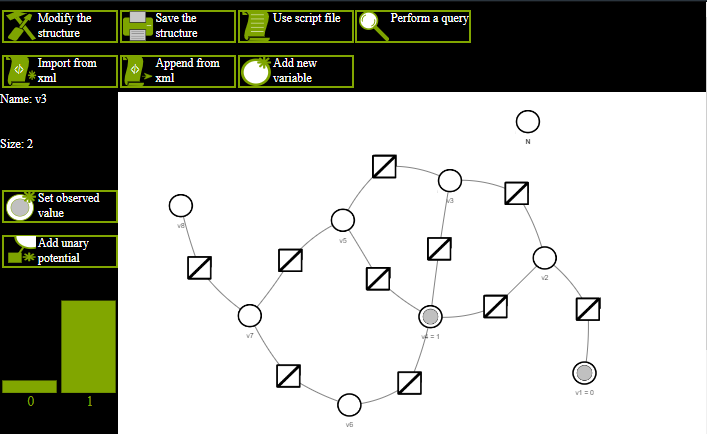
\includegraphics[width= \columnwidth]{../src/Chapter_additional/04_EFG_GUI/image/img_12.png}
\end{minipage}
\end{tabular}
	\caption{The inspector options for an hidden variable.}
	\label{fig:hidden}
\end{figure}

\subsection{Evidence variable}

When you click on an observed variable (case a in the right picture of Figure \ref{fig:inspector}) no further options will be available in the inspector.
